\documentclass[authordate, empirical,issue]{jote-new-article}

\usepackage{caption}

\usepackage{tabularx}

\usepackage{graphicx}

\usepackage{hyperref}

\usepackage[backend=biber,style=apa]{biblatex}


\PassOptionsToPackage{absolute,overlay}{textpos}
\RequirePackage{xcolor}
\usepackage{tikz}

\addbibresource{bibliography.bib}

\jotetitle{Prenatal sildenafil and fetal-placental programming in human pregnancies complicated by fetal growth restriction: A retrospective gene expression analysis}
\keywordsabstract{fetal growth restriction, sildenafil, developmental programming, RNA-sequencing, gene set enrichment analysis, human umbilical cord vein endothelial cells, placenta}
\abstracttext{\textbf{Objective:} Fetal growth restricted (FGR) offspring are more susceptible to develop cardiovascular and renal disease. The potential therapeutic value of sildenafil to improve fetal growth has recently been evaluated in several randomized clinical trials. Here we investigate whether administration of sildenafil during pregnancies complicated by FGR influences fetal-placental programming profiles, especially related to cardiorenal development and disease.
\vskip0pt
\textbf{Methods: }We collected human umbilical vein endothelial cells (HUVECs) and placental tissue within the Dutch STRIDER trial, in which sildenafil versus placebo treatment were randomly assigned to pregnancies complicated by severe early-onset FGR. Differential expression of genes of these samples were studied by whole genome RNA-sequencing. In addition, we performed gene set enrichment analysis focused on cardiovascular and renal gene sets to examine differentially expressed gene sets related to cardiorenal development and health.
\vskip0pt
\textbf{Results:} Our study showed similar gene expression profiles between treatment groups in HUVECs (n=12 sildenafil; n=8 placebo) and placentas (n=13 per group). Prenatal sildenafil exposure did not change cardiovascular or renal programming in pregnancies complicated by FGR. In placental tissue, prenatal sildenafil altered a few gene sets involved with the nitric oxide pathway potentially reflecting the mechanism of action of sildenafil. Prenatal sildenafil also upregulated gene sets related to immune pathways in placental tissue.
\vskip0pt
\textbf{Conclusions:} Overall, our study showed that sildenafil has the potential to alter placental (but not fetal) expression of gene sets related to immune pathways and did not support (in)direct reprogramming of cardiovascular or renal health in human pregnancies complicated by FGR.}

\runningauthor{Terstappen et al.}
\jname{Journal of Trial \& Error}
\jyear{2023}
\paperreceived{March 30, 2023}
\author[1]{\mbox{Fieke Terstappen\orcid{0000-0002-6587-1320}}}
\affil[1]{University Medical Center Utrecht, Wilhelmina Children's Hospital, Department of Obstetrics, Utrecht, The Netherlands}
\corremail{\href{mailto:F.Terstappen@umcutrecht.nl}{F.Terstappen@umcutrecht.nl}}
\corraddress{University Medical Center Utrecht}
\runningauthor{Terstappen et al.}
\author[2]{\mbox{Torsten Plösch\orcid{0000-0002-9305-4045}}}
\affil[2]{University Medical Center Groningen, Department of Obstetrics and Gynaecology, University of Groningen, Groningen, The Netherlands.}
\author[3,4]{\mbox{Jorg J.A. Calis}}
\affil[3]{University Medical Center Utrecht, Department of Cardiology, Utrecht, The Netherlands.}
\affil[4]{University Medical Centre Utrecht, Center for Translational Immunology, Utrecht, The Netherlands}
\author[5]{\mbox{Wessel Ganzevoort\orcid{0000-0002-7243-2115}}}
\affil[5]{Amsterdam University Medical Centers, Department of Obstetrics, University of Amsterdam, Amsterdam, The Netherlands}
\author[5]{\mbox{Anouk Pels}}
\author[1]{\mbox{Nina D. Paauw\orcid{0000-0003-3608-7083}}}
\author[2]{\mbox{Sanne J. Gordijn\orcid{0000-0003-3915-8609}}}
\author[6]{\mbox{Bas B. van Rijn\orcid{0000-0003-1305-3825}}}
\affil[6]{Erasmus MC University Medical Center Rotterdam, Department of Obstetrics and Fetal Medicine, Rotterdam, The Netherlands}
\author[3]{\mbox{Michal Mokry\orcid{0000-0002-5298-4852}}}
\author[1]{\mbox{A. Titia Lely\orcid{0000-0001-6356-7707}}}
\paperaccepted{August 23, 2023}
\paperpublished{September 26, 2023}
\paperpublisheddate{2023-09-26}
\jwebsite{https://journal.trialanderror.org}
\paperdoi{10.36850/e16}

\setcounter{page}{107}
\jissue{2}
\jvolume{4}
\jpages{107-121}
\specialissue{Scientific Failure and Uncertainty in the Health Domain}
\articletype{Special Issue - Empirical}

\begin{document}
\begin{frontmatter}
  \maketitle
  \begin{abstract}
    \printabstracttext
  \end{abstract}
\end{frontmatter}

\begin{figure*}
  \begin{fullwidth}
    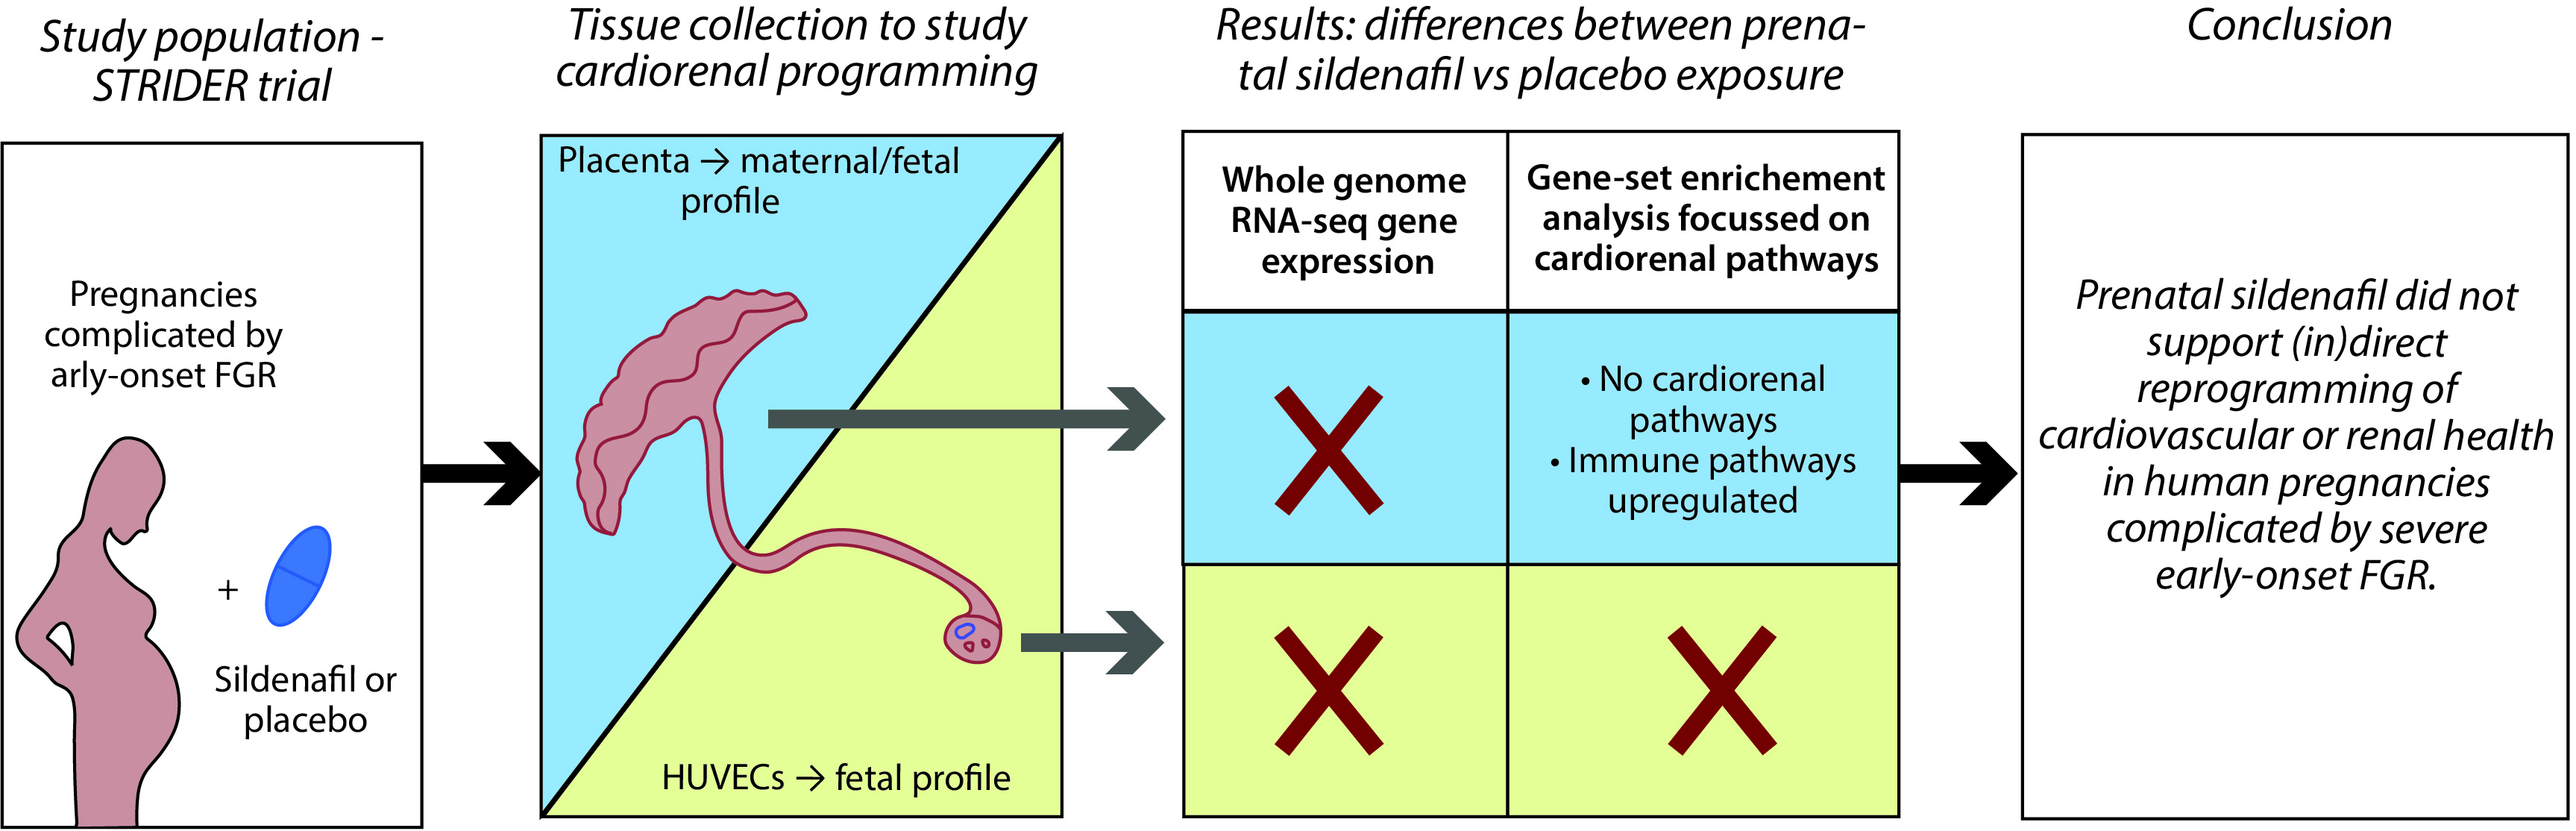
\includegraphics[width=\linewidth]{media/graphicalabstract.jpg}
    \caption*{Graphical abstract}
  \end{fullwidth}
\end{figure*}

\begin{takeHomeMessage}
  Fetal growth restriction (FGR) predisposes to cardiorenal diseases later in life. Prenatal administration of sildenafil showed beneficial effects on cardiovascular health in animal FGR offspring. However, this study did not support the potency of sildenafil to reprogram the cardiorenal health in human pregnancies complicated by FGR.
\end{takeHomeMessage}



\begin{tikzpicture}[remember picture, overlay]
    \node[align=left, text width=15cm, anchor=north west] 
    at ([xshift=4.7cm, yshift=-0.3cm]current page.north west) 
    {
        \noindent{\textbf{Correction notice}} \\
        Incorrect Special Issue Labeling (Article erroneously excluded): This article was previously not labeled as part of a special issue due to an error. This has now been corrected.\vspace{2pt}
        \noindent{{\color{joteorange}\rule{\linewidth}{1pt}}}
    };
\end{tikzpicture}


\lettrine{F}{etal} growth restriction (FGR) describes the inability of the fetus to reach its intrinsic growth potential. Early-onset FGR is most commonly caused by maternal vascular malperfusion resulting in placental insufficiency; a reduced uteroplacental blood flow impairs oxygen and nutrient supply towards the fetus s (Burton \& Jauniaux, 2018). Multiple lines of evidence suggest that exposure to this unfavorable intrauterine environment results in fetal adaptations, impaired maturation of organ development, and triggers developmental programming of cardiorenal diseases later in life (Barker, 2006; Sundrani et al., 2017; Chen \& Zhang, 2012; Henriksen \& Clausen, 2002). FGR offspring, and their future generations, are more susceptible to develop cardiovascular and renal disease, including hypertension, ischemic heart disease, chronic kidney disease and end-stage renal disease in adulthood (Malhotra et al., 2019; White et al., 2009; Gjerde et al., 2020; Kooiman et al., 2020; Demicheva \& Crispi, 2014; Dötsch et al., 2016; Sehgal et al., 2020; Nüsken et al., 2020). Adverse developmental programming might underlie this increased risk (Sehgal et al., 2020; Nüsken et al., 2020). A recent study showed altered gene expression and gene sets related to cardiovascular health and renal development in human umbilical vein endothelial cells (HUVECs) between placental insufficiency-induced FGR and control (Terstappen et al., 2020).



Mitigation of the detrimental developmental programming of cardiorenal disease following FGR in pregnancy is desirable e (Paauw et al., 2016). Several animal studies provided proof-of-concept of \emph{in utero }interventions to diminish adverse developmental programming, also known as reprogramming. For instance administration of nitric oxide (NO) stimulating agents during pregnancy improved cardiovascular outcomes alongside altered epigenetics and gene expression in fetuses or offspring of FGR models in rat, guinea pig or chicken (Herrera et al., 2017; Itani et al., 2017; Man et al., 2020; Z. Wu et al., 2015).



Sildenafil is one of these potential candidates to improve fetal growth and reprogram cardiorenal disease. Prenatal administration of this phosphodiesterase-5 showed beneficial effects on cardiovascular function in FGR models in rats, mice, and chickens (Itani et al., 2017; Mills et al., 2018; Terstappen et al., 2019). This might be a result of indirect influence on developmental programming, via improved fetal growth by uteroplacental blood flow by NO induced relaxation of the placental vascular bed on both the maternal and fetal side (Krause et al., 2011; Wareing et al., 2006).. In addition, the long-term benefit might also result from direct protection of developmental programming, since improvements in long-term cardiovascular function were also observed in a chick embryo model (without the presence of a placenta) of FGR after administration of sildenafil (Itani et al., 2017). While several animal and small-scaled human studies indeed showed improved fetal growth in the sildenafil-treated group (Paauw et al., 2017; Von Dadelszen et al., 2011), a series of randomized clinical trials (Sildenafil TheRapy In Dismal Prognosis Early-onset Fetal Growth Restriction [STRIDER]) designed within an international network did not show increased birth weight in pregnancies complicated with severe early-onset FGR following sildenafil compared to placebo (Pels et al., 2020; Sharp et al., 2018; Groom et al., 2019). These human data make indirect influence on developmental programming less likely; nevertheless, prenatal sildenafil could still directly influence developmental programming.



We collected HUVECs and placental tissue as a sub-study within the Dutch STRIDER trial to study whether sildenafil influences programming by regulation of fetal and placental gene expression. Hereby we aimed to address potential mechanisms underlying the effects of sildenafil on cardiovascular and renal programming in severe early-onset FGR offspring. Our approach involved whole genome RNA-sequencing to map differential expression per gene and gene set enrichment analysis focussed on cardiovascular and renal development, function and health.







\section{Methods}







\subsection{Study population}



For this substudy, women with a pregnancy complicated by severe early-onset FGR most likely based on placental insufficiency and participating in the Dutch STRIDER were recruited from the University Medical Center Utrecht (UMCU) and the Academic Medical Center (AMC) in Amsterdam from 09-07-2016 to 30-10-2017. In the Dutch STRIDER study, women were randomized to either prenatal administration of placebo or sildenafil at a dose of 25mg three times per day (Pels et al., 2020; Pels et al., 2017). The study population was selected based on low biometric parameters for gestational age and signs of placental insufficiency; inclusion and exclusion criteria have been described in detail previously (Pels et al., 2020; Pels et al., 2017). For this sub-study, we excluded cases in whom the offspring was diagnosed with a congenital disorder after birth.



The Dutch STRIDER trial (Clincial trial.gov identifier NCT02277132) was approved by the medical ethical committee of the AMC on 02-07-2014; protocol number 2014-131. The UMCU approved the study on 14-09-2015; protocol number 15-510/G-C. Prior to delivery, the STRIDER participants in this sub-study gave additional written informed consent for placental research (amendment approved on 29-01-2016, updated on 05-09-2017). The Dutch STRIDER study was halted mid-term because the interim-analysis showed futility in combination with potentially increased risk of mortality and persistent pulmonary hypertension (PPHN) in neonates.







\subsection{Clinical data }



Clinical data has been derived from the Dutch STRIDER database and patient records. The maternal medication was noted, including the start and duration of administration of the allocated drug. Unblinding of treatment allocation was done after all methods below were executed. Exact percentiles for weight and head circumference at birth were determined with Intergrowth-21\textsuperscript{st} (Anderson et al., 2016). Neonatal survival during hospital admission and cases of PPHN were registered.







\subsection{HUVECs isolation and RNA isolation }



Directly after placental delivery, the umbilical cord was stored in phosphate-buffered saline (PBS) solution (pH 7.2) at 4°C. HUVECs isolation occurred as previously described, preferably within 12 hours, but always within 24 hours after placental delivery (Hartman et al., 2020). We collected umbilical cords in both UMCU and AMC. Cannulation of the umbilical vein at one end allowed access for further processing. After washing with sterile PBS (pH 7.4; Gibco by Life Technologies, Grand Island, NY) the umbilical cord was clamped at both sides to incubate with accutase (0.02 µg/ml DNase; Innovative cell technologies Inc, San Diego, CA) for 5 minutes in 37°C sterile PBS to detach the endothelial cells. The detached HUVECs in accutase were flushed out of the umbilical vein with endothelial cell growth medium-2 (97\% EGM-2; basal medium and SingleQuots supplement [1.9\% FBS, 0.04\% hydrocortisone, 0.4\% hFGF-B2, 0.1\% vascular endothelial growth factor, 0.1\% R3-IGF-1, 0.1\% ascorbic acid, 0.1\% hEGF, 0.1\% GA-1000, 0.1\% heparin], Lonza Bioscience, Walkersville, MD) and centrifuged for 5 minutes at 330g at room temperature. The pellet was resuspended in 600 μl RA1 lysis buffer (Macherey-Nagel, Düren, Germany) and 6 μl 1M DTT and stored at -80°C until RNA isolation.



RNA was isolated using NucleoSpin RNA® (Macherey-Nagel), with RNA elution in 40 μl nuclease-free water. RNA concentration was quantified using Qubit RNA HS assay and Qubit fluorometer (ThermoFisher).







\subsection{RNA isolation of placental tissue}



Biopsies (4 by 4 mm) were taken from the middle of five cotyledons per placenta directly after birth and only in AMC. RNAlater stabilization solution (ThermoFisher Scientific) was used to freeze the (unrinsed) placental biopsies in liquid nitrogen and stored at -80°C until RNA isolation.

Frozen placenta samples were homogenized with a Tissuelyzer LT (Qiagen, Venlo, the Netherlands) in lysis buffer. Total RNA was isolated with the allprepRNA mini kit (Qiagen), following the manufacturer's protocol. RNA quality and quantity were characterized by a Nanodrop 2000c (Thermo Scientific, Pittsburgh, PA, USA). RNA was stored at -80°C until further analysis.







\subsection{RNA-sequencing of HUVECs and placental tissue}



Samples with a measurable amount (minimal concentration 41.4 ng/µl in placental samples and 2.1 ng/µl in HUVEC samples) of RNA were selected for RNA sequencing. Polyadenylated mRNA was isolated using Poly(A) beads (NEXTflex). Sequencing libraries were prepared by using the Rapid Directional RNA-seq kit (NEXTflex). The library was sequenced at the Utrecht Sequencing Facility (USEQ) on a Nextseq500 platform (Illumina) using a single-end 75-base pair high-output run. Reads were aligned to the human reference genome (GRCh37) using STAR version 2.4.2a. Read groups were added to the BAM files with Picard's AddOrReplaceReadGroups (v1.98). The BAM files were sorted with Sambamba v0.4.5, and transcript abundances were quantified with HTSeq-count version 0.6.1p117 using the union mode.







\subsection{Gene set analysis }



Gene set enrichment testing was performed on the hallmark (H), canonical pathway (C2-CP) and GO term (C5) gene set collections from the Molecular Signatures Database (version 7.1) (D.
Wu \& Smyth, 2012; Liberzon et al., 2016). Only gene sets with relation to renal or cardiovascular development or pathologies, or Nitric Oxide (NO) signaling were selected from the GO term gene sets (\textbf{\href{https://journal.trialanderror.org/pub/prenatal-sildenafil-pregnancies\#supplementary-materials}{Table S1}}). Gene sets with less than five genes in the set of selected genes (based on expression, see above) were excluded from the analysis, eventually resulting in 2,167 included gene sets







\subsection{Statistical analysis}



\subsubsection{Clinical data}



IBM SPSS Statistics 25 for Windows (version 25, UBM Corp, Armonk, NY) was used for statistical analysis. Parametric data tested with independent t-test are presented as mean ± SD, non-parametric data tested with Mann-Whitney are presented as median (minimum-maximum), and nominal data tested with Fisher exact are presented as n (\%). A two-sided p-value of below 0.05 was considered statistically significant.


\subsubsection{Differential expression of genes}



Read counts per gene, per sample, were analyzed for global expression differences using R (version 3.5.3). Genes were selected with an expression of one count per million reads (CPM) in at least 8 samples (n=13,760 genes selected). Read counts were Trimmed Mean of M-values (TMM)-normalized using the calcNormFactors function from the edgeR package (version 3.24.3) (Robinson et al., 2010). TMM-normalized counts were used to assess global transcriptional profile differences of all samples by Principal Comonent Analysis (PCA) (ten components). Ten Principal components (PC) were analyzed in the PCA analysis, values from each PC were checked for correlation to sample characteristics by the Mann-Whitney U test implemented in the scipy package (version 0.19.0) in python (version 2.7.10). Low-quality samples were identified and removed when passing any of these conditions: 1) number of reads were less than 1,000,000, 2) number of non-zero genes were less than 10,000, or 3) a combination of number of non-zero genes between 10,000-12,000 and being a visible outlier on one of the PCA components. HUVECs and placental tissue were analyzed separately.



Differential gene expression analysis was performed with the edgeR package (version 3.24.3) in R (version 3.5.3, R Core team, Auckland, New Zealand). Gene expression was modeled using the glmQLFit function in EdgeR (Robinson et al., 2010), to a model that included treatment group variables, as well as factors to capture mode of delivery (caesarean section vs spontaneous delivery), sex (male vs female), and gestational stage (preterm vs term) related gene expression variation. Differential gene expression was determined between treatment groups (sildenafil vs placebo) and the differential expression statistics were obtained using the glmQLFTest functionality in edgeR. False Discovery Rates (FDR) were determined using the Benjamini-Hochberg method to adjust for multiple testing and were considered significant when below 0.1 (in combination with unadjusted p-value <0.05; (Benjamini \& Hochberg, 1995).







\subsubsection{Differential expression of gene sets}



Gene set enrichment testing was performed with Correlation Adjusted MEan Rank (CAMERA), using the same linear model and contrasts as in the differential gene expression analysis (see above), and FDR were determined using the Benjamini-Hochberg method to adjust for multiple testing, which were considered significantly different when below 0.1 (Benjamini \& Hochberg, 1995). When a module showed ≥ 50\% overlap with higher ranking gene sets we only selected the more significant gene set. Heatmap for the gene sets related to the cardiovascular, renal and nitric oxide pathway were created.







\section{Results}







\subsection{Sample inclusion}



We collected umbilical cords from 14 sildenafil-treated and 10 placebo-treated births. Two sildenafil-treated and one placebo-treated sample did not yield enough RNA to perform RNA-sequencing. Therefore 12 sildenafil and 9 placebo HUVECs samples were used for RNA-sequencing. From the HUVECs samples, we excluded 1 low-quality run from the placebo group that was also an outlier in the RNA-seq data. Therefore, we proceeded with analyzing 12 sildenafil-treated versus 8 placebo-treated HUVEC samples.



We collected 16 sildenafil-treated and 18 placebo-treated placental biopsies. The RNA concentration of one placebo sample was too low to perform RNA-sequencing and thereby excluded. We also excluded one placental tissue sample in the placebo group based on postnatal detection of congenital disorders (Silver Russell syndrome). This resulted in 16 sildenafil versus 16 placebo-treated placental samples for RNA-sequencing. In these results, we identified three low-quality samples outliers in both the sildenafil and placebo group. Thus, we proceeded with 13 sildenafil-treated and 13 placebo-treated placenta samples for analysis.







\subsection{Study characteristics }



Patient characteristics are presented in \textbf{Table 1}. Birth weight did not differ between groups. Neonatal survival during hospital admission was approximately 20\% higher in the sildenafil group compared to the placebo group (not significantly different). Only sildenafil-exposed neonates suffered from PPHN during admission (n=3 in HUVECs samples and n=2 in the placental tissue samples).







\subsection{Differential expression of genes }



Principal component analysis (PCA) plots did not reveal clear clustering of sildenafil versus placebo in HUVECs (\textbf{Figure 1A}) or placental tissue (\textbf{Figure 1B}). The heatmaps supported that the gene expression between samples were similar (\textbf{\href{https://journal.trialanderror.org/pub/prenatal-sildenafil-pregnancies\#supplementary-materials}{Figure S1}}). Multidimensional scaling (MDS) plots of HUVECs material showed clustering in prematurity as potential modifier, but not in the treatment group, delivery route, or sex (\textbf{\href{https://journal.trialanderror.org/pub/prenatal-sildenafil-pregnancies\#supplementary-materials}{Figure S2}}). MDS plots of placental material showed no clustering in the treatment group, sex, prematurity or delivery route as potential modifiers (\textbf{\href{https://journal.trialanderror.org/pub/prenatal-sildenafil-pregnancies\#supplementary-materials}{Figure S3}}). All of the study characteristics were tested for association for all of the first 10 PCs. Gestational stage was associated with PC2 and PC5 in HUVECs and PC8 in placenta, delivery route was associated with PC2 and PC5 in HUVECs and PC1 and PC10 in placenta, and sex was associated with PC3 in HUVECs and PC8 in placenta (\textbf{\href{https://journal.trialanderror.org/pub/prenatal-sildenafil-pregnancies\#supplementary-materials}{Table S2}}). Therefore, differences in expression due to mode of delivery, gestational stage, and sex were accounted for in the modeling of gene expression.



The analysis of differential expression of genes, including genes involved in the NO pathway or related to cardiovascular or renal development or function, did not show any significant differences between the treatment groups, neither in HUVECs samples (\textbf{\href{https://journal.trialanderror.org/pub/prenatal-sildenafil-pregnancies\#supplementary-materials}{Table S3}}) nor in placenta samples (\textbf{\href{https://journal.trialanderror.org/pub/prenatal-sildenafil-pregnancies\#supplementary-materials}{Table S4}}).


\subsection{Differential expression of gene sets}



Gene set enrichment analysis did not show any differences between treatment groups in HUVECs samples (\textbf{\href{https://journal.trialanderror.org/pub/prenatal-sildenafil-pregnancies\#supplementary-materials}{Table S5}}). However, in placental samples 90 gene sets were upregulated in sildenafil-treated compared to placebo-treated (\textbf{\href{https://journal.trialanderror.org/pub/prenatal-sildenafil-pregnancies\#supplementary-materials}{Table S6}}). The selection of only the highest-ranking gene set module (overlapping modules excluded) resulted in 64 upregulated gene sets and 5 downregulated gene sets. These gene sets mostly involved immune pathways, and three gene sets were related to the NO pathway and one to cardiovascular disease (\textbf{Table 2}). Heatmaps were made for the top ten gene sets related to immune pathways (\textbf{\href{https://journal.trialanderror.org/pub/prenatal-sildenafil-pregnancies\#supplementary-materials}{Figure S4}}), and the four gene sets related to the NO pathway and cardiovascular disease (\textbf{\href{https://journal.trialanderror.org/pub/prenatal-sildenafil-pregnancies\#supplementary-materials}{Figure S5}}). This was done to study the extent of up- and downregulation for the distinct genes in these gene sets in each sample and were ordered per duration of treatment. From this analysis, most genes were up- and downregulated in accordance with the differential gene set analysis results for immunity, but this did not apply for gene sets related to the NO pathway and cardiovascular disease. None of the heatmaps showed ascending or descending expression levels correlating to duration of treatment.



The adverse \emph{in utero }environment resulting in fetal growth restriction (FGR) predisposes the offspring to develop cardio-renal disease beyond the fetal developmental phase by altered epigenetic programming. Interest grew in prenatal administration of sildenafil after several animal studies showed improved fetal growth and long-term cardiovascular function.



\section{Discussion}







This sub-study within the Dutch STRIDER trial evaluated whether prenatal sildenafil administration during pregnancies complicated by severe early-onset FGR influenced gene modules, with specific focus on cardiovascular and renal programming. The RNA expression in collected HUVECs and placental tissue did not differ between the sildenafil or placebo group. Gene set enrichment analysis also showed no differences in gene sets related to cardiovascular and renal health in HUVECs, but three gene sets involved in the NO-pathway and one in cardiovascular health were possibly different in placenta samples. Additionally, we observed an upregulation of several gene sets related to immune pathways in the sildenafil-exposed placental samples.







\subsection{Lack of difference in gene expression and gene sets related to cardiorenal health}



The results of the three STRIDER trials in UK, New-Zealand and the Netherlands suggested that prenatal sildenafil does not have an indirect programming effect via placental function improvements since they observed no beneficial effects on pregnancy outcomes, such as birth weight, prolongation of pregnancy, or perinatal morbidity or mortality (Groom et al., 2019; Sharp et al., 2018; Pels et al., 2020). Complementary to this, the results from this current sub-study showed no direct cardiovascular or renal programming following prenatal sildenafil exposure. The low sample size due to the mid-term halt of the study and only collecting samples in part of the participating centers due to logistics might both have limited detection of beneficial effects. Alternatively, our lack of clear results regarding cardiovascular and renal programming might be a result of interspecies differences, since several animal studies did report a reprogramming potential of prenatal administration of NO-stimulating agents (sildenafil, pentaerythritol tetranitrate, N-acetely cysteine) in animal models for placental insufficiency (Herrera et al., 2017; Itani et al., 2017; Z. Wu et al., 2015). However, a recent study showed that prenatal sildenafil reprogrammed salt-sensitive hypertension in rat FGR offspring, but had not affected renal function nor did they find differences in targeted RNA-seq data in renal tissue (Turbeville et al., 2020). These conflicting results might plead for the use of tissue collected from complicated pregnancies (such as FGR) in humans to study developmental programming on a molecular level rather than the use of animal tissue.







\subsection{Upregulated gene sets involved with NO pathway }



We observed upregulation of three gene sets related to the NO pathway (response to \emph{v}ascular endothelial growth factor stimuli, leukocyte adhesion to vascular endothelial cells, and negative regulation of the NO metabolic process) in placental tissues in the sildenafil group compared with the placebo group. These gene sets might reflect the mechanism of action of sildenafil. Preclinical studies report conflicting results, with some showing altered expression of metabolites in the NO-pathway after sildenafil exposure in fetal cardiac or lung tissue (Itani et al., 2017; Shue et al., 2014), while others did not find these differences in expression in spite of beneficial functional effects (George et al., 2013). However, while these gene sets were significantly different in our study, the heatmaps of these gene sets showed that the differences of the individual genes were minimal and independent of duration of sildenafil intake. Therefore, these inconclusive results did not lead to a clear insight regarding the mechanism of action of sildenafil.



The Dutch STRIDER trial showed a potentially increased risk of PPHN in neonates (Pels et al., 2020). The gene set of increased leukocyte adhesion to vascular endothelial cells combined with our gene set's result on immune pathways might suggest that this pathway is involved in the increased PPHN risk (Rafikov et al., 2019; Kuebler et al., 2018; El Chami \& Hassoun, 2012; Kobayashi et al., 2004). However, this was not observed in HUVECs representing the fetal profile. To gain better insight into underlying mechanisms involved with the potentially increased risk of PPHN in the Dutch STRIDER trial requires follow-up studies that were beyond the scope of this study.







\subsection{Upregulated gene sets involved in the immune pathway }



Interestingly, sildenafil administration resulted in the upregulation of several gene sets involved in immune or inflammation pathways and, additionally, longer sildenafil intake correlated with higher expression of genes related to these pathways. Pregnancies complicated by placental insufficiency syndromes show an increased placental release of pro-inflammatory cytokines, such as TNF-α and IL-6 and therefore targeting inflammation has been of therapeutic interest (George \& Granger, 2011; Oyston et al., 2015; Kniotek \& Boguska, 2017). Sildenafil might exert an anti-inflammatory response by inhibition of TNF-α and IL1β release and stimulation of IL-10 release (Ribaudo et al., 2016; Kniotek \& Boguska, 2017). Indeed, prenatal sildenafil reduced TNF-α levels in maternal plasma and placenta in the rat model for preeclampsia and FGGR (Gillis et al., 2016) and reduced placental TNF-α and IL1β in the mice model for pregnancy loss. Administration of a different NO stimulating agent during healthy pregnancy lowered placental expression of IL1β and IL18 in sows (Luo et al., 2019). Our study showed only significant upregulation of the IL-10 signaling and pathway, but not TNF- α or IL1β. We speculate that most of the significantly upregulated gene sets promote protection to auto-immunity and innate immunity, which is necessary for embryonal implantation and placentation. This could potentially contribute to reducing pregnancy loss after prenatal sildenafil treatment when used earlier in pregnancy (Luna et al., 2015).




\begin{originalPurpose}
  The adverse \emph{in utero }environment resulting in fetal growth restriction (FGR) predisposes the offspring to develop cardio-renal disease beyond the fetal developmental phase by altered epigenetic programming. Interest grew in prenatal administration of sildenafil after several animal studies showed improved fetal growth and long-term cardiovascular function.

  An international STRIDER consortium emerged to evaluate the therapeutic potency of sildenafil to improve fetal growth in pregnancies complicated by FGR. In our sub-study (of the Dutch STRIDER trial) we aimed to study whether prenatal sildenafil influences developmental programming of cardiorenal health by examining whole genome RNA-sequencing and gene set enrichment analysis in human umbilical vein endothelial cells and placental tissue. We hypothesized that prenatal sildenafil alters fetal-placental programming profiles especially related to cardiorenal development and disease.

  The interim-analysis of the Dutch STRIDER trial showed futility in combination with potentially increased mortality and morbidity in neonates. Hereafter all trials and inevitably our substudy were halted. This made our sub-study the first and last to investigate whether prenatal sildenafil administration in pregnancies complicated by FGR could influence fetal-placental programming of cardiorenal health.

  Our study does not support the use of prenatal sildenafil for cardiorenal reprogramming. This is contrary to several animal studies, which may be suggestive of interspecies differences. Our results might be reassuring considering the negative clinical results of the STRIDER study and highlight the need for tissue collection from complicated pregnancies in humans to study developmental programming on a molecular or genetic level.
\end{originalPurpose}


\subsection{Strengths and limitations}



To our knowledge, this is the first study examining the effect of prenatal sildenafil administration during human pregnancies complicated by early-onset FGR on programming. One major strength is that we used two different types of tissue - with placenta representing maternal profile and HUVECs representing fetal profile - collected from a well-defined randomized controlled trial with severe early-onset FGR.



We acknowledge some limitations. This was a sub-study in which we collected samples from live births from the Dutch STRIDER trial and therefore does not fully represent the clinical pregnancy outcomes. We attempted to minimize samples bias selection by using all the samples available, even if they were not paired. Because of the halt of the Dutch STRIDER study and because women were only recruited for this substudy in 2 of the 11 recruiting centers, this study is limited by a relatively low sample size. However, it also made the analysis of these samples unique and valuable. We used native HUVECs without prior selective culturing to be as close as possible to the in situ situation. Despite extensive washing, HUVEC samples might therefore have been contaminated with a few other fetal blood cells.







\section{Conclusion and future perspectives}



FGR is associated with the developmental programming of cardiovascular and renal diseases later in life. Currently, no therapy exists to improve fetal growth or prevent these detrimental long-term consequences. Administration of PDE-5 inhibitors such as sildenafil during pregnancy showed beneficial effects on cardiovascular health in animal FGR offspring. However, our study in human pregnancies complicated by severe early-onset FGR did not show an effect of prenatal sildenafil administration on cardiovascular or renal programming. Future research is needed to understand whether an interspecies difference underlies these discrepancies or other differences in study design (such as dose) between animal and human studies. In order to progress, elucidation of (direct or indirect) underlying mechanisms and safety studies are of paramount importance in the evaluation of any new potential intervention.



\section{List of abbreviations}



CAMERA, Correlation Adjusted MEan RAnk; CPM, count per million reads; EGM, endothelial cell growth medium; FDR, False Discovery Rates; FGR, fetal growth restriction; GA, gestational age; GSEA, gene set enrichment analysis; HELLP, Hemolysis, Elevated Liver enzymes and Low Platelet syndrome; HUVECs, human umbilical vein endothelial cells; IL1β, Interleukin 1β; MDS, Multidimensional scaling; MgSO\textsubscript{4}, magnesium sulfate; NO, nitric oxide; PC, principle components; PCA, principal components analysis; PBS, phosphate-buffered saline; PPHN, persistent pulmonary hypertension; STRIDER, Sildenafil TheRapy In Dismal Prognosis Early-onset Fetal Growth Restriction; TMM, Trimmed mean of M-values; TNF-α, Tumor necrosis factor; VEGF, vascular endothelial growth factor.















\section{Ethics approval and consent to participate}



The Dutch STRIDER trial (Clinical trial.gov identifier NCT02277132) was approved by the medical ethical committee of the AMC on 02-07-2014; protocol number 2014-131. The UMCU approved the study on 14-09-2015; protocol number 15-510/G-C. Prior to delivery, the STRIDER participants in this sub-study gave additional written informed consent for placental research (amendment approved on 29-01-2016, updated on 05-09-2017).







\section{Conflict of interest}



None declared.



\section{Availability of data and materials}



The datasets generated and/or analyzed during the current study are not publicly available due to the Dutch privacy law to protect participants, but are partly and always coded available from the corresponding author on request. All data generated or analyzed during this study are included in this published article and its supplementary information files.

\section{References}

Anderson, N. H., Sadler, L. C., McKinlay, C. J. D., \& McCowan, L. M. E. (2016). INTERGROWTH-21st vs customized birthweight standards for identification of perinatal mortality and morbidity. \emph{American Journal of Obstetrics and Gynecology, 214}(4), 509 1–509 7.

Barker, D. (2006). Adult consequences of fetal growth restriction. \emph{Clinical Obstetrics and Gynecology, 49}, 270–83.

Benjamini, Y., \& Hochberg, Y. (1995). Controlling the false discovery rate: A practical and powerful approach to multiple testing. \emph{Journal of the Royal Statistical Society: Series B (Methodological), 57}(1), 289–300.

Burton, G. J., \& Jauniaux, E. (2018). Pathophysiology of placental-derived fetal growth restriction. \emph{American Journal of Obstetrics and Gynecology, 218}(2), 745–761. \url{https://doi.org/10.1016/j.ajog.2017.11.577}

Chen, M., \& Zhang, L. (2012). Epigenetic mechanisms in developmental programming of adult disease. Drugs Discovery Today, 16, 1007–1018. Demicheva, E., \& Crispi, F. (2014). Long-term followup of intrauterine growth restriction: Cardiovascular disorders. \emph{Fetal Diagnosis and Therapy, 36}(2), 143–153.

Dötsch, J., Alejandre-Alcazar, M., Janoschek, R., Nüsken, E., Weber, L. T., \& Nüsken, K. D. (2016). Perinatal programming of renal function. \emph{Current Opinion in Pediatrics, 28}(2), 188–194. \url{https://doi.org/10.1097/MOP.0000000000000312}

El Chami, H., \& Hassoun, P. (2012). Immune and inflammatory mechanisms in pulmonary arterial hypertension. \emph{Progress in Cardiovascular Diseases, 55}(2), 218–228. \url{https://doi.org/10.1038/jid.2014.371}

George, E. M., \& Granger, J. P. (2011). Mechanisms and potential therapies for preeclampsia. \emph{Current Hypertension Reports, 13}(4), 269–275.

George, E. M., Palei, A. C., Dent, E. A., \& Granger, J. P. (2013). Sildenafil attenuates placental ischemiainduced hypertension. \emph{American Journal of Physiology. Regulatory, Integrative and Comparative Physiology, 305}(4), 397–403.

Gillis, E. E., Mooney, J. N., Garrett, M. R., Granger, J. P., \& Sasser, J. M. (2016). Sildenafil treatment ameliorates the maternal syndrome of preeclampsia and rescues fetal growth in the dahl salt-sensitive rat. \emph{Hypertension, 67}(3), 647–653.

Gjerde, A., Lilla, B. S., Marti, H., Reisæter, A. V., \& Vikse, B. E. (2020). Intrauterine growth restriction, preterm birth and risk of end-stage renal disease during the first 50 years of life. \emph{Nephrology Dialysis Transplantation, 35}(7), 1157–1163.

Groom, K., McCowan, L. M., Mackay, L. K., Lee, A. C., Gardener, G., Unterscheider, J., Sekar, R., Dickinson, J. E., Muller, P., Reid, R. A., Watson, D., Welsh, A., Marlow, J., Walker, S. P., Hyett, J., Morris, J., Stone, P. R., \& Baker, P. N. (2019). STRIDER NZAus: multicentre randomised controlled trial of sildenafil therapy in early-onset fetal growth restriction. \emph{BJOG, 126}(8), 997–1006.

Hartman, R. J. G., Kapteijn, D. M. C., Haitjema, S., Bekker, M. N., Mokry, M., Pasterkamp, G., Civelek, M., \& Ruijter, H. M. D. (2020). \emph{Intrinsic transcriptomic sex differences in human endothelial cells at birth and in adults are associated with coronary artery disease targets}. Scientific Reports.

Henriksen, T., \& Clausen, T. (2002). The fetal origins hypothesis: Placental insufficiency and inheritance versus maternal malnutrition in wellnourished populations. \emph{Acta Obstetricia et Gynecologica Scandinavica, 81}(2), 112–114.

Herrera, E. A., Cifuentes-Zúñiga, F., Figueroa, E., Villanueva, C., Hernández, C., Alegría, R., Arroyo-Jousse, V., Penaloza, E., Farias, M., Uauy, R., Casanello, P., \& Krause, B. J. (2017). Nacetylcysteine, a glutathione precursor, reverts vascular dysfunction and endothelial epigenetic programming in intrauterine growth restricted guinea pigs. \emph{The Journal of Physiology, 595}(4), 1077–1092.

Itani, N., Skeffington, K. L., Beck, C., \& Giussani, D. A. (2017). Sildenafil therapy for fetal cardiovascular dysfunction during hypoxic development: Studies in the chick embryo. \emph{Journal of Physiology, 595}(5), 1563–1573.

Kniotek, M., \& Boguska, A. (2017). Sildenafil can affect innate and adaptive immune system in both experimental animals and patients. \emph{Journal of Immunology Research}, 4541958.

Kobayashi, H., Yamataka, A., Okazaki, T., Lane, G. J., Puri, P., \& Miyano, T. (2004). Increased levels of circulating adhesion molecules in neonates with congenital diaphragmatic hernia complicated by persistent pulmonary hypertension. \emph{Pediatric Surgery International, 20}(1), 19–23. \url{https://doi.org/10.1007/s00383-003-1072-8}

Kooiman, J., Terstappen, F., van Wagensveld, L., Franx, A., Wever, K. E., Roseboom, T. J., Joles, J. A., Gremmels, H., \& Lely, A. T. (2020). Conflicting effects of fetal growth restriction on blood pressure between human and rat offspring. \emph{Hypertension, 75}(3), 806–818.

Krause, B. J., Hanson, M. A., \& Casanello, P. (2011). Role of nitric oxide in placental vascular development and function. \emph{Placenta, 32}(11), 797–805.

Kuebler, W. M., Bonnet, S., \& Tabuchi, A. (2018). Inflammation and autoimmunity in pulmonary hypertension: Is there a role for endothelial adhesion molecules? \emph{Pulmonary Circulation, 8}(2). \url{https://doi.org/10.1177/2045893218757596}

Liberzon, A., Birger, C., Ghandi, M., Jill, P., Tamayo, P., Jolla, L., \& Jolla, L. (2016). \emph{MSigDB H collection, 1}(6), 417–425.

Luna, R. L., Nunes, A. K. S., Oliveira, A. G. V., Araujo, S. M. R., Lemos, A. J. J. M., Rocha, S. W. S., Croy, B. A., \& Peixoto, C. A. (2015). Sildenafil (viagra®) blocks inflammatory injury in LPS-induced mouse abortion: A potential prophylactic treatment against acute pregnancy loss? \emph{Placenta, 36}(10), 1122–1129.

Luo, Z., Xu, X., Sho, T., Luo, W., Zhang, J., Xu, W., Yao, J., \& Xu, J. (2019). Effects of n-acetyl-cysteine supplementation in late gestational diet on maternalplacental redox status, placental NLRP3 inflammasome, and fecal microbiota in sows. \emph{Journal of Animal Science, 97}(4), 1757–1771.

Malhotra, A., Allison, B., Castillo-Melendez, M., Jenkin, G., Polglase, G., \& Miller, S. (2019). Neonatal morbidities of fetal growth restriction: Pathophysiology and impact. \emph{Frontiers in Endocrinology, 10}(55).

Man, A. W. C., Chen, M., Wu, Z., Reifenberg, G., Daiber, A., Münzel, T., Xia, N., \& Li, H. (2020). Renal effects of fetal reprogramming with pentaerythritol tetranitrate in spontaneously hypertensive rats. \emph{Frontiers in Pharmacology, 11}(April), 1–13.

Mills, V., Plows, J. F., Zhao, H., Oyston, C., Vickers, M. H., Baker, P. N., \& Stanley, J. L. (2018). Effect of sildenafil citrate treatment in the eNOS knockout mouse model of fetal growth restriction on longterm cardiometabolic outcomes in male offspring. \emph{Pharmacological Research, 137}(September), 122–
134.

Nüsken, E., Fink, G., Lechner, F., Voggel, J., Wohlfarth, M., Sprenger, L., Mehdiani, N., Weber, L. T., Liebau, M. C., Brachvogel, B., Dotsch, J., \& Nüsken, K. D. (2020). Altered molecular signatures during kidney development after intrauterine growth restriction of different origins. \emph{Journal of Molecular Medicine, 98}(3), 395–407. \url{https://doi.org/10.1007/s00109-020-01875-1}

Oyston, C. J., Stanley, J. L., \& Baker, P. N. (2015). Potential targets for the treatment of preeclampsia. \emph{Expert Opinion on Therapeutic Targets, 19}(11), 1517–1530.

Paauw, N. D., Terstappen, F., Ganzevoort, W., Joles, J. A., Gremmels, H., \& Lely, A. T. (2017). Sildenafil during pregnancy: A preclinical meta-analysis on fetal growth and maternal blood pressure. \emph{Hypertension, 70}(5), 998–1006.

Paauw, N. D., van Rijn, B. B., Lely, A. T., \& Joles, J. A. (2016). Pregnancy as a critical window for blood pressure regulation in mother and child: Programming and reprogramming. \emph{Acta Physiologica, 219}(1), 241–259.

Pels, A., Derks, J., Elvan-Taspinar, A., van Drongelen, J., de Boer, M., Duvekot, J., van Laar, J., van yck, J., Al-Nasiry, S., Sueters, M., Post, M., Onland, W., van Wassenaer-Leemhuis, A., Naaktgeboren, C., Jakobsen, J. C., Gluud, C., Duijnhoven, R. G., Lely, T., Gordijn, S., \& Group, D. S. T. R. I. D. E. R. T. (2020). Maternal sildenafil vs placebo for severe early-onset fetal growth restriction: A randomized clinical trial. \emph{JAMA Network Open, 6}, 1–14.

Pels, A., Kenny, L. C., Alfirevic, Z., Baker, P. N., von Dadelszen, P., Gluud, C., Kariya, C. T., Mol, B. W., Papageorghiou, A. T., van Wassenaer-Leemhuis, A. G., Ganzevoort, W., Groom, K. M., \& international STRIDER Consortium. (2017). STRIDER (sildenafil therapy in dismal prognosis early onset fetal growth restriction): An international consortium of randomised placebo-controlled trials. \emph{BMC Pregnancy Childbirth, 17}(440), 1–8.

Rafikov, R., Nair, V., Sinari, S., Babu, H., Sullivan, J. C., Yuan, J. X. J., Desai, A. A., \& Rafikova, O. (2019). Gender difference in damage-mediated signaling contributes to pulmonary arterial hypertension. \emph{Antioxidants and Redox Signaling, 31}(13), 917–932. \url{https://doi.org/10.1089/ars.2018.7664}

Ribaudo, G., Angelo Pagano, M., Bova, S., \& Zagotto, G. (2016). New therapeutic applications of phosphodiesterase 5 inhibitors (PDE5-is. \emph{Current Medicinal Chemistry, 23}(12), 1239–1249. 

Robinson, M. D., McCarthy, D. J., \& Smyth, G. K. (2010). Edger: A bioconductor package for differential expression analysis of digital gene expression data. \emph{26}(1), 139–40.

Sehgal, A., Alexander, B. T., Morrison, J. L., \& South, A. M. (2020). Fetal growth restriction and hypertension in the offspring: Mechanistic links and therapeutic directions. \emph{The Journal of Pediatrics, 224}, 115–123.

Sharp, A., Cornforth, C., Jackson, R., Harrold, J., Turner, M. A., Kenny, L. C., N., B. P., Johnstone, E. D., Khalil, A., von Dadelszen, P., Papageorghiou, A. T., Alfirevic, Z., \& group, S. T. R. I. D. E. R. (2018). Maternal sildenafil for severe fetal growth restriction (STRIDER): A multicentre, randomised, placebocontrolled, double-blind trial. \emph{The Lancet Child and
Adolescent Health, 2}(2), 93–102.

Shue, E. H., Schecter, S. C., Gong, W., Etemadi, M., Johengen, M., Iqbal, C., Derderian, S. C., Oishi, P., Fineman, J. R., \& Miniati, D. (2014). Antenatal maternally-administered phosphodiesterase type 5 inhibitors normalize eNOS expression in the fetal lamb model of congenital diaphragmatic hernia. \emph{Journal of Pediatric Surgery, 49}(1), 39–45.

Sundrani, D., Roy, S., Jadhav, A., \& Joshi, S. (2017). Sex-specific differences and developmental programming for diseases in later life. \emph{Reproduction, F, 29}, 2085–2099.

Terstappen, F., Calis, J. J. A., Paauw, N. D., Joles, J. A., van Rijn, B. B., Mokry, M., Plosch, T., \& Lely, A. T. (2020). Developmental programming in human umbilical cord vein endothelial cells following fetal growth restriction. \emph{Clinical Epigenetics, 12}(1), 185.

Terstappen, F., Spradley, F. T., Bakrania, B. A., Clarke, S. M., Joles, J. A., Paauw, N. D., Garrett, M. R., Lely, A. T., \& Sasser, J. M. (2019). Prenatal sildenafil therapy improves cardiovascular function in fetal growth restricted offspring of dahl salt-sensitive rats. \emph{Hypertension, 73}(5), 1120–1127.

Turbeville, H. R., Johnson, A. C., Garrett, M. R., \& Sasser, J. M. (2020). Sildenafil citrate does not reprogram risk of hypertension and chronic kidney disease in offspring of preeclamptic pregnancies in the dahl SS/jr rat. \emph{Kidney360, 1}(6), 510–520. \url{https://doi.org/10.34067/kid.0001062020}

Von Dadelszen, P., Dwinnell, S., Magee, L., Carleton, B. C., Gruslin, A., Lee, B., Lim, K. I., Liston, R. M., Miller, S. P., Rurak, D., Sherlock, R. L., Skoll, M. A., Wareing, M. M., \& Baker, P. N. (2011). Sildenafil citrate therapy for severe early-onset intrauterine growth restriction. \emph{Research into Advanced Fetal Diagnosis and Therapy Group Baker, P. N}(5), 624–628.

Wareing, M., Myers, J. E., O’Hara, M., Kenny, L. C., Taggart, M. J., Skillern, L., Machin, I., \& Baker, P. N. (2006). Phosphodiesterase-5 inhibitors and omental and placental small artery function in normal pregnancy and pre-eclampsia. \emph{European Journal of Obstetrics, Gynecology, and Reproductive Biology, 127}(1), 41–49.

White, S. L., Perkovic, V., Cass, A., Chang, C. L., Poulter, N. R., Spector, T., Haysom, L., Craig, J. C., Al Salmi, I., Chadban, S. J., \& Huxley, R. R. (2009). Is low birth weight an antecedent of CKD in later life? a systematic review of observational studies. \emph{American Journal of Kidney Diseases, 54}(2), 248–261.

Wu, D., \& Smyth, G. K. (2012). Camera: A competitive gene set test accounting for inter-gene correlation. \emph{Nucleic Acids Research, 40}(17), 133.

Wu, Z., Siuda, D., Xia, N., Reifenberg, G., Daiber, A., Munzel, T., Fostermann, U., \& Li, H. (2015). Maternal treatment of spontaneously hypertensive rats with pentaerythritol tetranitrate reduces blood pressure in female offspring. \emph{Hypertension, 65}(1), 232–237.




\clearpage
\onecolumn
\section{Figure legends}











\begin{figure}[h!]
  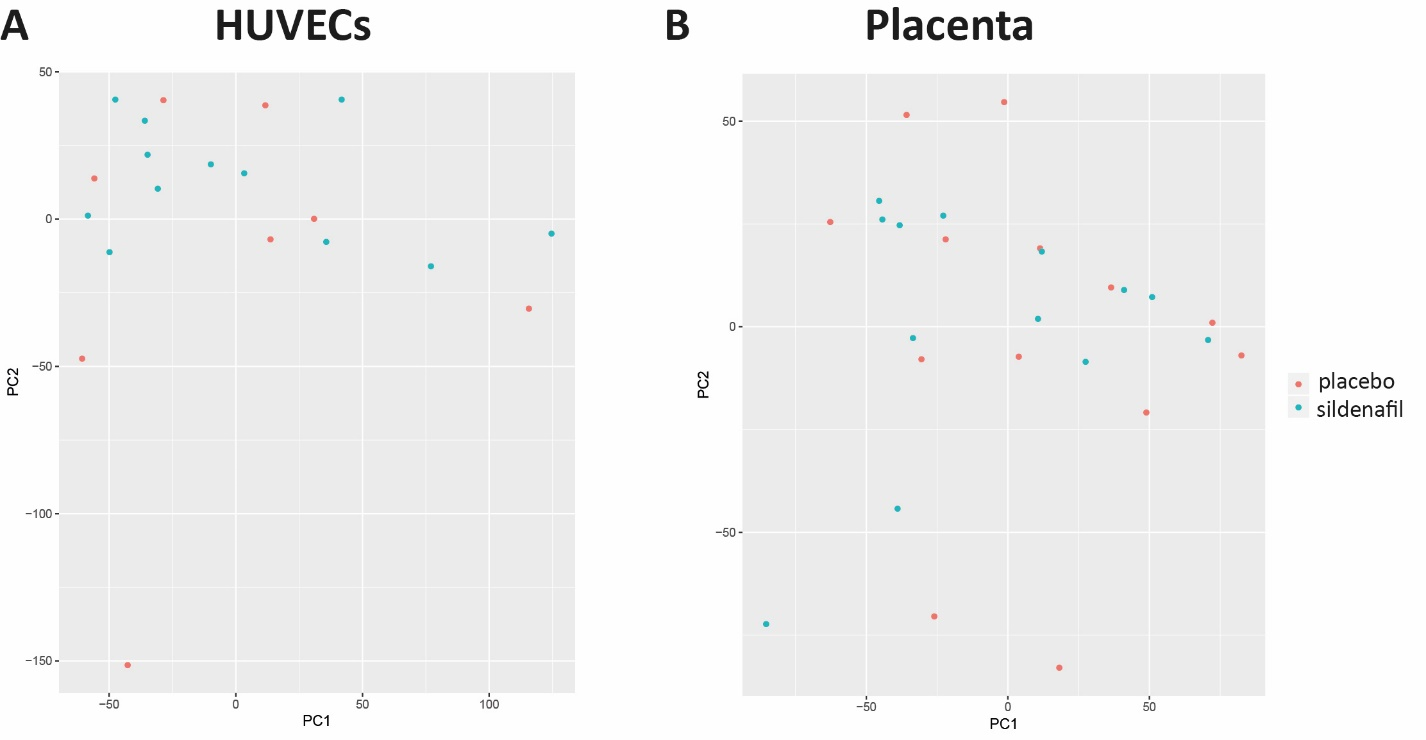
\includegraphics[width=\linewidth]{media/image1.jpeg}

  \caption{Principal component analysis (PCA) plots of A) human umbilical vein endothelial cells (HUVECs) and of B) placenta.PC1 versus PC2 does not show clustering in treatment group sildenafil (blue) vs. placebo (red) in HUVECs or placental tissue.}

  \label{fig:rId8}


\end{figure}





\newpage

\section{Tables}


\begin{table}[h!]
  \begin{fullwidth}
    \caption{Maternal and neonatal characteristics}
    \footnotesize

  \resizebox{\linewidth}{!}{%
    \begin{tabular}{@{} l l l l l l l l l l l l l l l l l l l l l l l l @{}}

                                                                & \multicolumn{3}{l}{\textbf{HUVECs}} & \multicolumn{3}{l}{\textbf{Placenta}}
      \\

                                                                & \textbf{Sildenafil}\textbf{(n=12)}  & \textbf{Placebo}\textbf{(n=8)}        &
      \textbf{p-value}                                          & \textbf{Sildenafil}\textbf{(n=13)}  & \textbf{Placebo (n=13)}
                                                                & \textbf{p-value}                                                                                                                  \\
      \midrule
      \multicolumn{7}{@{}l}{\textbf{Maternal characteristics during pregnancy}}                                                                                                                     \\

      Age, years                                                & 35±6                                & 31±3                                  & 0.19   & 34±6                     & 33±6     & 0.66 \\

      (pre-pregnancy) BMI, kg/m\textsuperscript{3}              & 23±3                                & 24±6                                  & 0.74   & 24±4\textsuperscript{\#}
                                                                & 26±7\textsuperscript{\#}            & 0.29                                                                                        \\

      Preeclampsia/HELLP, \%                                    & 8 (67)                              & 3 (38)                                & 0.36   & 6 (46)                   & 5 (39)   & 1.00
      \\

      Smoking, \%                                               & 1 (8)                               & 0 (0)                                 & 1.00   & 1 (8)                    & 2 (15)   & 1.00 \\

      \multicolumn{7}{@{}l}{\textbf{Maternal medication during pregnancy}}                                                                                                                          \\

      Antihypertensive drugs, \%                                & 8 (67)                              & 2 (25)                                & 0.17   & 6 (46)                   & 4 (31)   &
      0.69                                                                                                                                                                                          \\

      Antenatal steroids, \%                                    & 9 (75)                              & 7 (88)                                & 0.62   & 8 (62)                   & 7 (54)   & 1.00
      \\

      MgSO\textsubscript{4}, \%                                 & 2 (18)\textsuperscript{\#}          & 0 (0)                                 & 0.49   & 2 (15)
                                                                & 0 (0)                               & 0.48                                                                                        \\

      GA start allocated drug, weeks                            & 25.0±2.0                            & 24.5±2.2\textsuperscript{\#}          &
      0.64                                                      & 24.0±2.5                            & 25.0±2.4                              & 0.33                                                \\

      Duration allocated drug, days                             & 30.6±20.1                           & 44.3±20.1\textsuperscript{\#}         &
      0.17                                                      & 25.4±18.5                           & 24.7±17.8                             & 0.92                                                \\

      \multicolumn{7}{@{}l}{\textbf{Delivery}}                                                                                                                                                      \\

      Caesarean section, \%                                     & 9 (75)                              & 6 (75)                                & 1.00   & 8 (62)                   & 6 (46)   & 0.70 \\

      Apgar at 5 min                                            & 8 (3-10)                            & 8 (6-10)                              & 0.88   & 6 (0-9)                  & 8 (0-10) & 0.29 \\

      \multicolumn{7}{@{}l}{\textbf{Neonatal characteristics}}                                                                                                                                      \\

      Male gender, \%                                           & 7 (58)                              & 5 (63)                                & 1.00   & 8 (62)                   & 6 (46)   & 0.70 \\

      GA at birth, weeks                                        & 30.8±4.3                            & 32.2±3.7                              & 0.45   & 27.8±1.9                 & 29.4±4.1 & 0.21
      \\

      Birth weight, gram                                        & 795 (430-2528)                      & 852 (580-2282)                        & 0.64   & 520(280-1005)
                                                                & 770 (315-2385)                      & 0.23                                                                                        \\

      Birth weight, percentile                                  & 3.6 (<0.01-16.7)                    & 1.0 (<0.01-4.7)                       & 0.22   & 0.1 (<0.01-13.3)
                                                                & 0.7(<0.01-8.0)                      & 0.19                                                                                        \\

      \emph{ - <3}\textsuperscript{\emph{rd}}\emph{ percentile} & 6 (50)                              & 2 (25)
                                                                & 0.37                                & 8 (62)                                & 8 (62) & 1.00                                       \\

      Survival, \%                                              & 8 (67)                              & 7 (88)                                & 0.60   & 5 (42)                   & 8 (62)   & 0.43 \\

      PPHN, \%                                                  & 3 (25)                              & 0 (0)                                 & 0.24   & 2 (15)                   & 0 (0)    & 0.48 \\

      \bottomrule                                                                                                                                                                                   \\
    \end{tabular}
    }

    Data expressed as mean±SD, median (min-max), and n(\%), which were respectively tested with independent t-test, Mann-Whitney, or Fisher exact. Magnesium sulfate (MgSO\textsubscript{4}) was based on the maternal indication. \textsuperscript{\# }represents missing data of maximal one patient per group and therefore, the percentages are calculated based on the number of observations/measurements. GA, gestational age; HELLP, Hemolysis, Elevated Liver enzymes and Low Platelet syndrome; HUVECs, human umbilical vein endothelial cells;\textsubscript{ }p, percentile; PPHN, persistent pulmonary hypertension.

  \end{fullwidth}
\end{table}


\begin{table}[h!]
  \begin{fullwidth}
    \caption{Significantly different gene sets related to cardiovascular development or NO pathway between \emph{\textbf{in vivo}}\textbf{sildenafil and placebo treated placental tissue samples}}

    \begin{tabularx}{\linewidth}{@{} X l l l X @{}}
      Gene set name                                                               & Up ordown                                                                                                   & p-value                                                                                                                                                      & FDR    & Brief description                                                                                                              \\

      GO\_CELLULAR\_RESPONSE\_TO\_VASCULAR\_ENDOTHELIAL\_GROWTH\_FACTOR\_STIMULUS & Up                                                                                                          &
      0.0013                                                                      & 0.0437                                                                                                      & Any process that results in a change in state or activity of a cell (movement, secretion, enzyme production, gene expression) as a result of a VEGF stimulus
      \\

      GO\_LEUKOCYTE\_ADHESION\_TO\_VASCULAR\_ENDOTHELIAL\_CELL                    & Up                                                                                                          & 0.0031                                                                                                                                                       & 0.0848
                                                                                  & The attachment of a leukocyte to vascular endothelial cell via adhesion molecules
      \\

      GO\_NEGATIVE\_REGULATION\_OF\_NITRIC\_OXIDE\_METABOLIC\_PROCESS             & Up                                                                                                          & 0.0031                                                                                                                                                       & 0.0848
                                                                                  & Any process that stops, prevents or reduces the frequency, rate or extent of nitric oxide metabolic process
      \\

      BIOCARTA\_AMI\_PATHWAY                                                      & Up                                                                                                          & 0.0036                                                                                                                                                       & 0.0945 & Acute myocardial infarction is the condition of irreversible necrosis of the heart muscle that results from prolonged ischemia
      \\
    \end{tabularx}
    Ordered according to lowest false discovery rate (FDR). VEGF, vascular endothelial growth factor\emph{.}
  \end{fullwidth}
\end{table}


\end{document}